\section{\texorpdfstring{Polynomial Hierarchy cont}{Polynomial Hierarchy cont}}
\vspace{5mm}
\large

\begin{consequence}[Polynomial hierarchy collapse]\label{ph_collapse}
	if $\Sigma_k = \Pi_k$ for some $k > 0$ then
	\[ \forall j \geq 0: \Sigma_{k + j} = \Pi_{k + j} = \Sigma_k \]
\end{consequence}
\begin{proof}
	By induction on j. For 0 is true by assumption.

	Induction step:
	\[ \Sigma_{k + j + 1} =^{c)} \exists \Pi_{k + j} =^{by\ I.H.} \exists \Sigma_{k + j} \]
	By c)
	\[ \exists \Sigma_{k + j} = \Sigma_{k + j} \]
	By I.H. again
	\[ \Sigma_{k + j} = \Sigma_k \]

	Similarly for $\Pi_{k + j + 1}$.
	% todo finish
	\[ \Pi_{k + j + 1} =^{f)} \forall \Sigma_{k + j} = \]
\end{proof}

\begin{consequence}
	Either $\forall k: \Sigma_k \subset \Sigma_{k + 1}$ or PH collapses.
\end{consequence}
\begin{proof}
	Assume
	\[ \Sigma_k = \Sigma_{k + 1} \]
	We know
	\[ \Sigma_{k + 1} = \TNP(\Sigma_{k}) = \TNP(\Pi_k) \supset \Pi_k \]
	Implies by assumption
	\[ \Pi_k \subseteq \Sigma_k \Rightarrow \Sigma_k = \Pi_k \]
	Then by \cref{ph_collapse} PH collapses after $k$.

	In particular for $k = 0$ we get
	\[ \TP = \TNP \Rightarrow PH = \TP \]
\end{proof}

\begin{consequence}
	\[ \exists k \in \N: \TP = \Sigma_0 \subset \Sigma_k \Rightarrow \TP \subset \TNP \]
\end{consequence}
\begin{proof}
	By reversing previous condition.
\end{proof}

\begin{definition}
	PSPACE-complete
\end{definition}

\begin{lemma}\label{ph_col_lemma}
	Let $L$ be $PS$-complete and $L \in \Sigma_k$ then $PH = \Sigma_k$.
\end{lemma}
\begin{proof}
	Take $L_2 \in PS$ by the polynomial reduction, since
	\[ \exists DTM\ M_d: x \in L_2 \iff M(x) \in L \]
	Also there is acceptor
	\[ \exists NTM\ M_n: L = L(M_n, D) \]
	for some $D \in \Sigma_{k - 1}$
	Then we construct new NTM by concatenation of $M_d$ and $M_n$.

	% todo join 2 proofs
	\[ L_2 \in PS \]
	Therefore
	\[ PS \subseteq \Sigma_k \]
	We already know that
	\[ PH \subseteq PS \]
	Therefore
	\[ PH = \Sigma_k \]
\end{proof}

\begin{consequence}
	if $PH = PS$ then
	\[ \exists k \in \N: PH = \Sigma_k \]

	Assuming that $\exists L \in PS$-complete.

	Which implies, that if PH grows infinitely and no PS-complete is in PH.
	Then $PS \setminus PH$ contains all $PS$-complete languages.
\end{consequence}
\begin{proof}
	We take L, by $PH = PS$
	\[ \exists k: L \in \Sigma_k \]
	then by lemma \cref{ph_col_lemma}
	\[ PH = PS \]
\end{proof}

\section{\texorpdfstring{PS-complete lang}{PS-complete lang}}
\vspace{5mm}
\large

\begin{definition}
	QBF - quantifiable boolean formula
	%todo
\end{definition}

\begin{definition}
	QBF problem
\end{definition}

How do we evaluate QBF with no free variables?
\begin{itemize}
	\item $ \exists x (E) \iff E_0 \lor E_1$
	\item $ \forall x (E) \iff E_0 \land E_1$
\end{itemize}
`
\begin{example}
	\[ \forall x (\forall x (\exists y (x \lor y)) \land \neg x) \]
	by rules above
	\[ (\forall x (\exists y (x \lor y)) \land \neg 0) \land (\forall x (\exists y (x \lor y)) \land \neg 1) \]
\end{example}

\begin{note}
	SAT - language of satisfiable CNFs.
	We can think of it as
	\[ \exists x_1 \exists x_2 \ldots \exists x_n (F(x_1, x_2, \ldots, x_n) \]
	Therefore SAT is a special case of QBF.
\end{note}

\begin{theorem}
	QBF is in PS.
\end{theorem}
\begin{proof}
	We construct DTM to evaluate QBF without free variables as following
	\begin{itemize}
		\item $\neg(E) \to$ evaluate E and negate all results
		\item $(E_0) \lor (E_1) \to $ evaluate $E_0$, $E_1$ then by disjunction
		\item $(E_0) \land (E_1) \to $ evaluate $E_0$, $E_1$ then by conjunction
		\item $\exists (E) \to$ compute $E_l, E_r$, then compute $E_l \lor E_r$
		\item $\forall(E) \to$ compute $E_l, E_r$, then compute $E_l \land E_r$
	\end{itemize}

	We have at most $n$ operators.
	We get binary tree that evaluates the formula.
	Where every branch is bounded by total length of initial formula.

	$\bigO(n^2)$ is enough space for evaluation.
\end{proof}

\begin{note}
	% todo replace by bigor
	\[ F = \bigcap (x_i \to y_i) = \bigcap (\neg x_i \lor y_j)\]
	The resulting formula is shortest CNF representing $F$.
	Length changed to $\Theta(n^2)$.

	Now 2nd formula
	\[ H = (\exists z) [(\bigcap(x_i \to z)) \land (\bigcap (z \to y_j))] \]
	which is linear. $H$ is an encoding of $F$ with auxiliary variables.
\end{note}

\begin{theorem}[QBF $\in$ PS-hard]
	QBF is in PS-hard (sketch).
\end{theorem}
\begin{proof}
	Every $L \in PS$ arbitrary can be reduces to QBF in poly time.

	By the definition of PS
	\[ \exists DTM\ M: L = L(M), \exists p(n) \]
	M accepts L in polynomial space $p(n)$.

	We have \[ 2^{c_m p(n)} \] configurations of M and every configuration can be encoded by string of length
	\[ c_m p(n) = m(n) := m \]
	We assume, that is only 1 accepting configuration.

	$x \in L \iff \exists $ path of length $m$ in \emph{configuration graph} from $C_0 \to C{acc}$.
	Use similar algorithm as in Savic theorem \cref{savic}, but encode computation in QBF.

	Notation, where $\phi$ is an encoding of allowed transition in Cook-Levin theorem.
	We construct QBF $\psi$.
	\begin{itemize}
		\item $ \psi_0(C, C^{\prime}) = 1 \iff \phi_m(C, C^{\prime})$ is satisfiable
		\item $ \psi_i(C, C^{\prime}) = 1 \iff $ there exists path $C \to C^{\prime}$ of length $2^i$
		\item $ \psi_m(C_0, C_{acc}) = 1 \iff x \in L$
	\end{itemize}

	Obvious idea that would not work
	\[ \psi_i(C, C^{\prime}) = \exists C_{int} (\psi_i(C, C_{int}) \land \psi_i(C_{int}, C^{\prime})) \]
	Since every such change doubles size of the formula, we end up with
	\[ |\psi_m| \in \Omega(2^m p(n)) \]

	Main idea
	\[ \psi_i(C, C^{\prime}) = \exists C_{int} \forall D_1, D_2 [(D_1 = C \land D_2 = C^{\prime}) \lor (D_1 = C_{int} \land D_2 = C^{\prime})] \Rightarrow \psi(D_1, D_2) \]
	Formally, implication could be replaced by $\neg x \lor y$.
	Now
	\[ |\psi_i| = |\psi_{i - 1}| + \bigO(1) \]
	Therefore
	\[ |\psi_m| = \bigO(m^2) \]
\end{proof}

\subsection{P-completeness}

\begin{note}
	If we use polynomial time reducibility, almost all languages(except trivial: empty and all words) are $\TP$-complete.

	Therefore we use a different reducibility.
\end{note}

\begin{definition}
	A is \emph{log-space} reducible to B if $\exists$ DTM transducer M that works in log space (excluding input and output tape).
	Such that $x \in A \iff M(x) \in B $.
\end{definition}

\begin{definition}
	L is $\TP$-complete $\iff L \in \TP \land \forall A \in \TP A$ is log-space reducible to L.
\end{definition}

\begin{theorem}[P-complete vs LOG]
	Let $L$ be $\TP$-complete and $L \in LOG = DS(\log(n)) \Rightarrow \TP = LOG$.
\end{theorem}
\begin{proof}
	\[ LOG \subseteq \TP \]
	We want
	\[ \TP \subseteq LOG \]

	Let $B \in \TP$ arbitrary, we need log-space acceptor for B $\Rightarrow B \in LOG$.
	From $L$ is $\TP$-complete $\Rightarrow \exists$ log-space DTM $M_L: x \in B \iff M_L(x) \in L$.
	From $L \in LOG \Rightarrow \exists $ log-space DTM acceptor $M_{log}: L = L(M_{log}) $.

	We cannot simply concatenate 2 machines, as output tape of the first machine $M_L$ becomes work tape of the 2nd.
	Output tape is not guaranteed to be log-space.
	Let $Y$ be the output of $M_L$
	\[ |Y| \leq 2^{c_M \log n} = n^{c_M} \]

	Idea: keep just current symbol on output of $M_L$ and the position.
	Then start the next step of $M_{log}$.
	Then restart $M_L$ and discard output with position $ < i$.
	Repeat.

	We need 2 counters $i, j \in \{ 1, \ldots, |Y| \}$.
	Which require
	\[ \log(n^c) = c \log n \]
	%One counter is incremented with write on output tape, other counter keeps position on the output tape.
	%while(work)
	%{
	%	for(j = 0; j < i; ++j)
	%	{
	%		if(
	%	}
	%}

	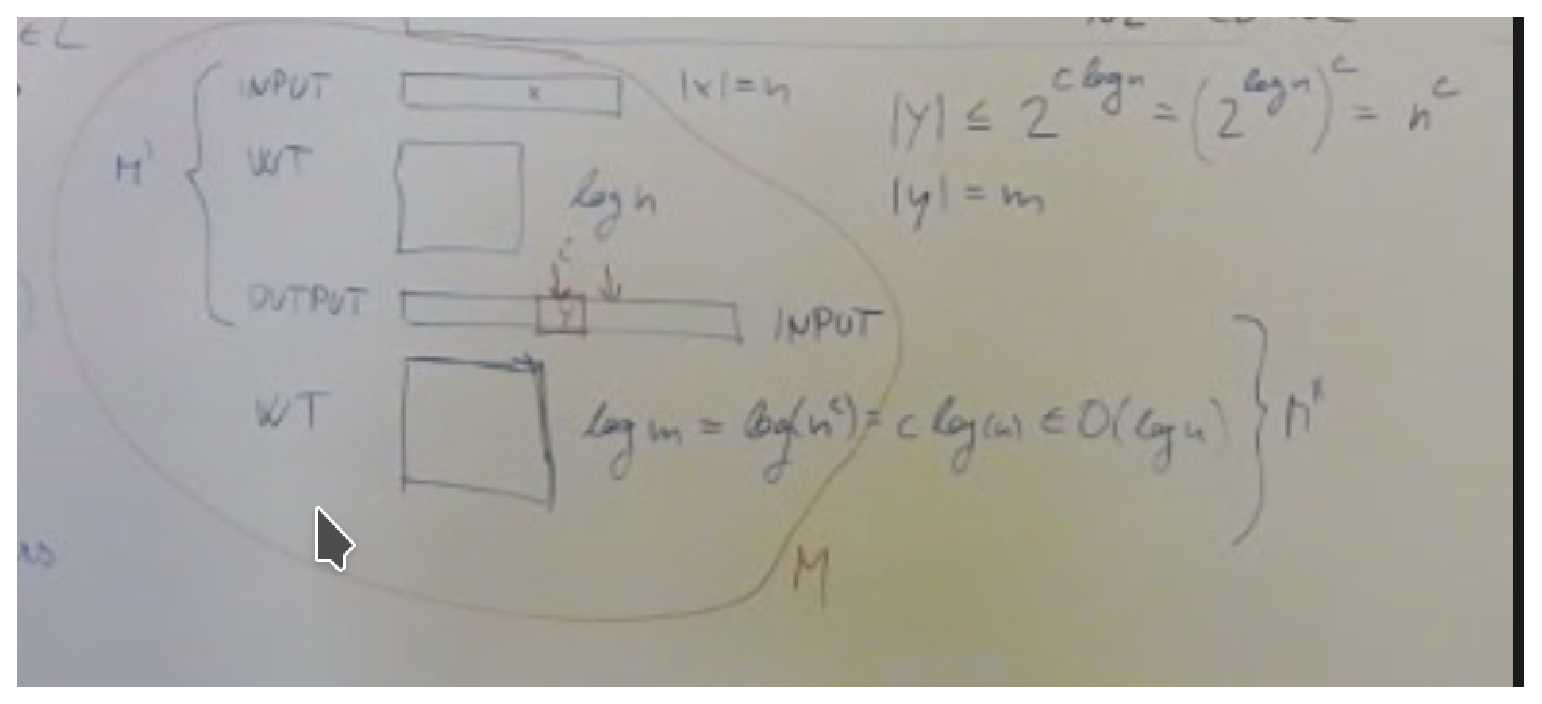
\includegraphics[scale=0.4]{p_nlog.eps}
\end{proof}

\begin{consequence}
	Let $L$ be $\TP$-complete and $L \in NLOG = NS(\log(n)) \Rightarrow \TP = NL$.

	Proof is same, but acceptor is non deterministic.
\end{consequence}

Question: what if we use log-space reducibility in $\TNP$-complete definition?
This is stricter, since if we can reduce in log-space, we can also reduce in polynomial time (by time and space comparison with $2^n$).

\begin{theorem}[Szelepcsenyi-Immerman]
	\[NL = co-NL \]
\end{theorem}
\begin{proof}
\end{proof}
